\section*{Practical 2: Implementing a Phase Space Sampler}
\addcontentsline{toc}{section}{Practical 2:  Implementing a Phase Space Sampler}


This week we will look at how phase space sampling can be implemented in python. We can begin by updating our repository with 
\begin{codeenv}
    git pull
\end{codeenv}
Make sure you're in the project directory when running this, else you'll get an error. If things aren't working (because you've done some edits), you can run
\begin{codeenv}
    git stash
\end{codeenv}
the stash away your changes. You can now \codeinline{git pull} again to get the latest version. You can then resync your changes on top of the new version using \codeinline{git stash apply}.
In the experiments folder, you should now have a new file, \codeinline{sampling_experiment.py}.
You should now also see that \codeinline{run.py} has been edited with a new case in \codeinline{__main__} for the sampling experiment. If we try and run this now, we might find that we're missing dependencies. To add the missing requirements, we can use the requirements file supplied by the repository:
\begin{codeenv}
    python3 -m pip install -r ./CHEP/requirements.txt
\end{codeenv}
Lets run the new experiment. To see how to use the new code, we can run
\begin{codeenv}
    python3 run.py sampling_experiment --help
\end{codeenv}
This tells us that we have optional run parameters which allows us to specify our random seed. Lets just run the code without a seed. If we wait a moment, we should see some lovely distributions similar to what we have seen in lectures! If the plots don't show (\codeinline{* UserWarning: FigureCanvasAgg is non-interactive}), try running 
\begin{codeenv}
    sudo apt-get install python3-tk
\end{codeenv}

\begin{figure}[H]
    \centering
    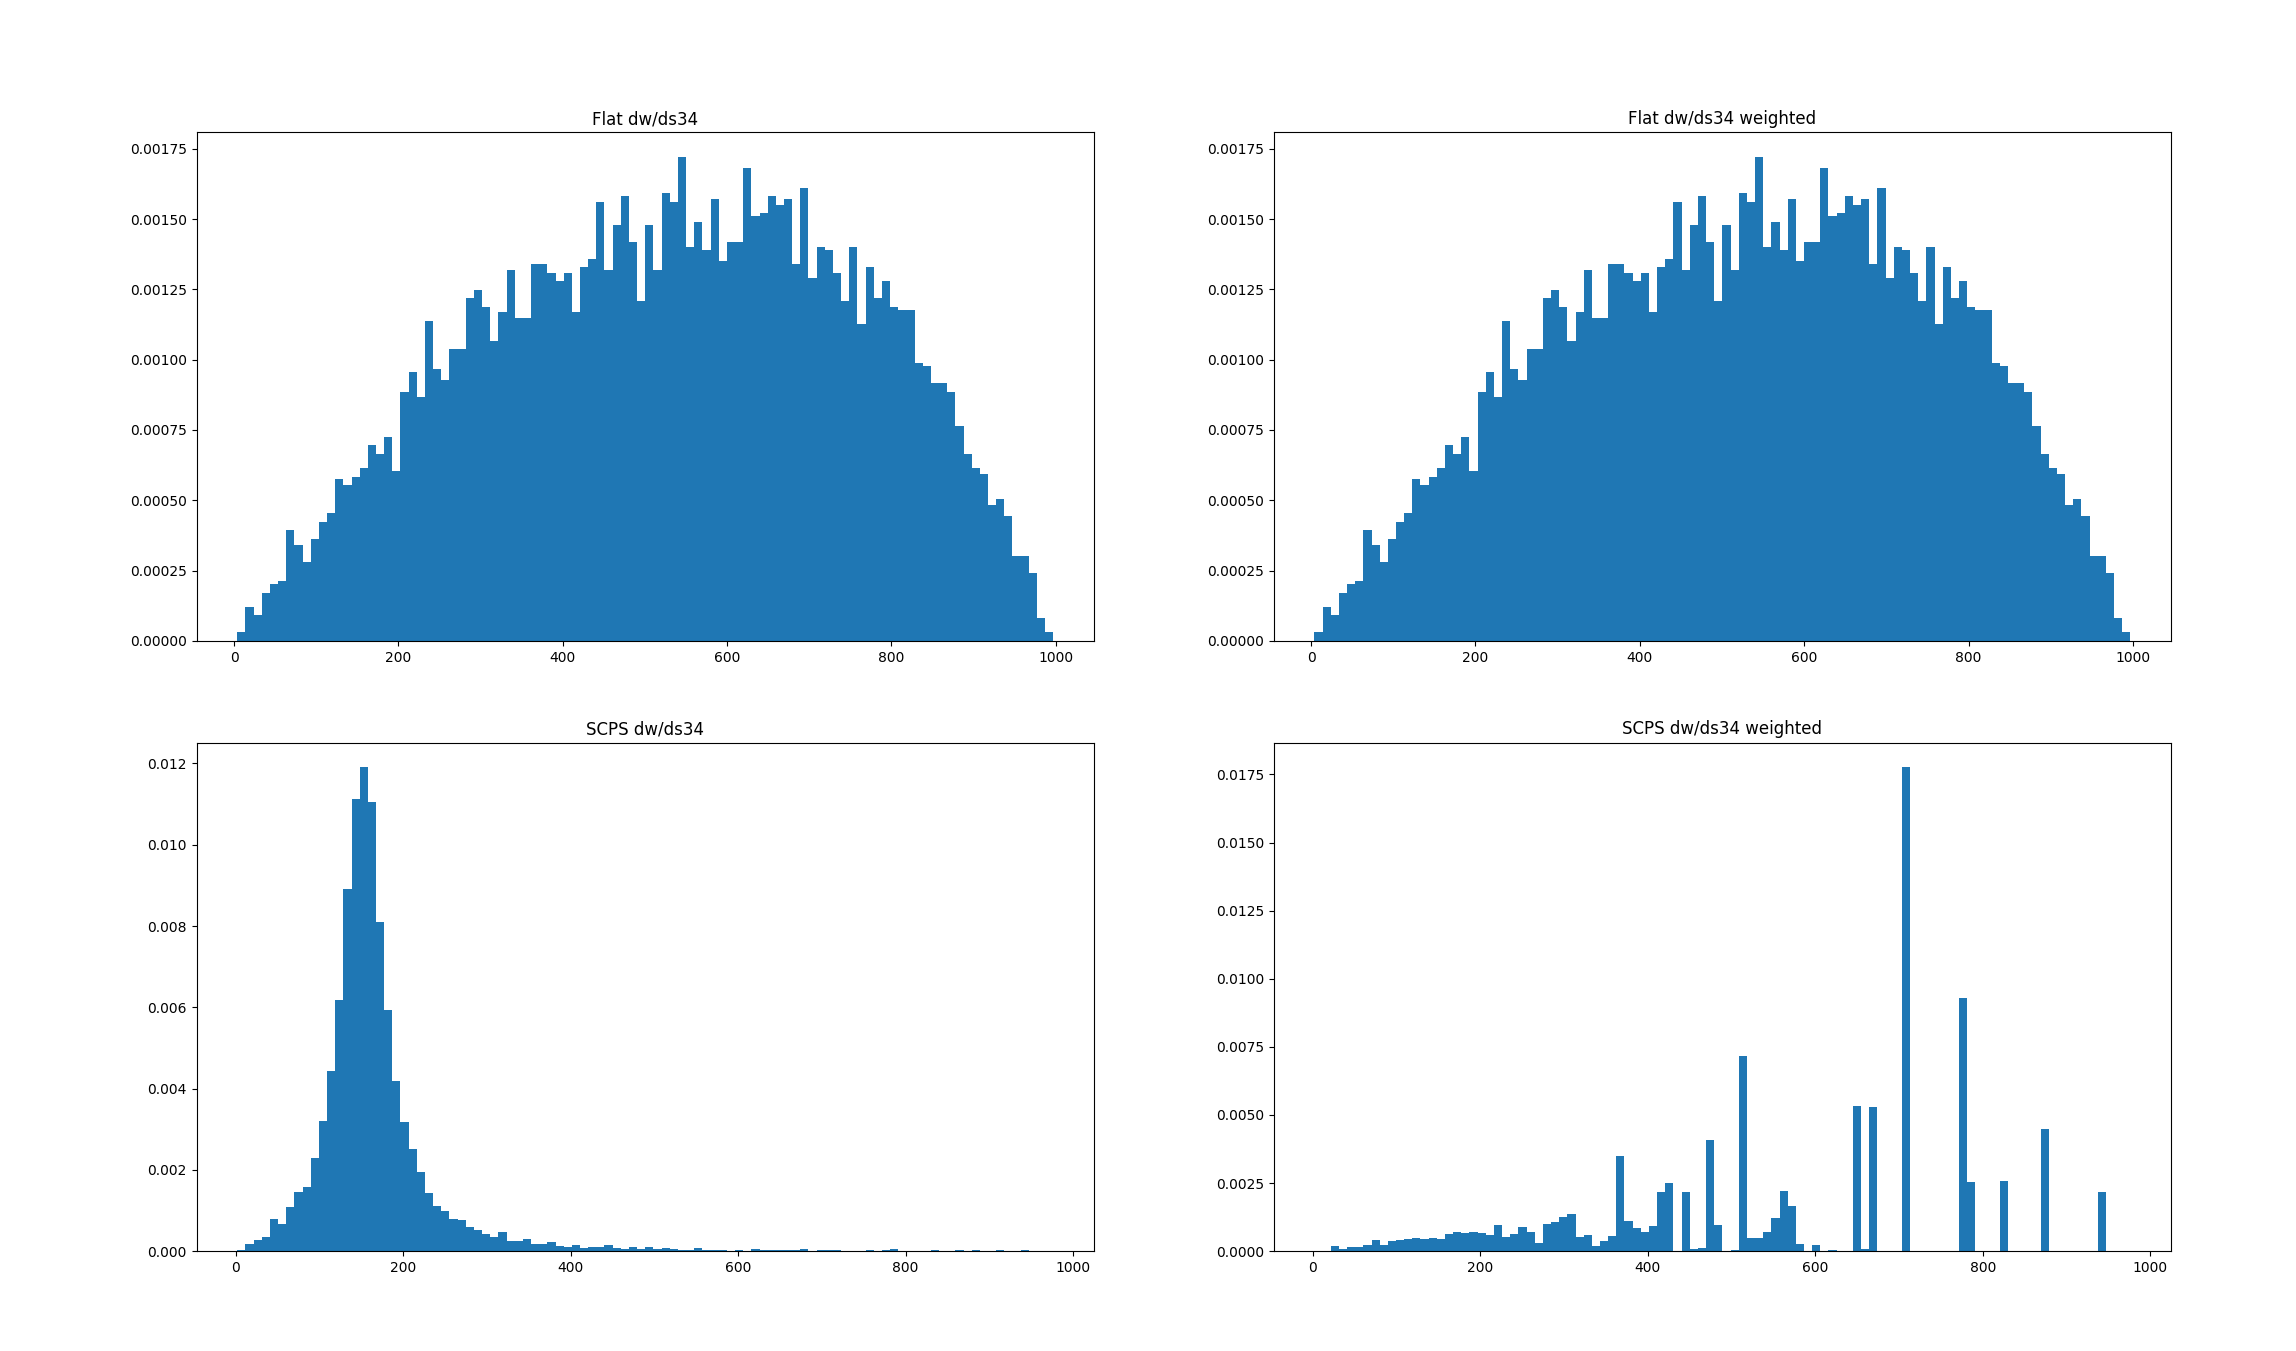
\includegraphics[width=0.75\linewidth]{tex/ims/phasespace1.png}
    \caption{Phase Space Sampling. The top row is ``flat space", so the right image is the left multiplied by the Jacobian which is just a constant (``$1$" for a normalised volume). The bottom row is biased sampling, to pick momenta distributed around the relevant pole of our process, in this case the $Z$ boson with mass 150GeV and width 60GeV.}
    \label{fig:enter-label}
\end{figure}


Lets try and understand what we're looking at, and what the code is doing. Lets open VSCode with \codeinline{code .}. Inside \codeinline{sampling_experiment}, firstly, the code picks a model. It then specifies the \codeinline{topology} - this corresponds to an assignment of momenta to our diagram.
\begin{center}
    \begin{tikzpicture}
    \begin{feynman}
        % Define vertices
        \vertex (e1) at (-3, 1) {\(e^-, p_{-3}\)};
        \vertex (e2) at (-3, -1) {\(e^+,  p_1\)};
        \vertex (v1) at (-1, 0.5) {};
        \vertex (v2) at (-1, -0.5) {};
        \vertex (v3) at (0,0.5);
        \vertex (mu1) at (2,1) {\(\mu^+,p_3\)};
        \vertex (mu2) at (2,0) {\(\mu^-,p_4\)};
        \vertex (photon) at (2, -1) {\(\gamma,p_5\)};

        % Define diagram
        \diagram* {
            (e1) -- [fermion] (v1) -- [fermion , edge label={$p_{-2}$}] (v2),
            (e2) -- [anti fermion] (v2),
            (v1) -- [boson, edge label={\(Z,\) $p_{-1}$}] (v3),
            (v3) -- [fermion] (mu2),
            (v3) -- [anti fermion] (mu1),
            (v2) -- [photon] (photon), % Initial-state radiation from the electron
        };
    \end{feynman}
\end{tikzpicture}
\end{center}

We have a propagator with momentum $p_1-p_5$ (t-channel). We also have an $s-$channel block. This is specified for our particular process in \codeinline{get_topology()}. You can \codeinline{Ctrl+Click} on  \codeinline{get_topology()} to see the assignment explicitly. Inside this function, for the outgoing $s-$channel,  we assign momentum 3 to particle ID $-12$ ($\mu^+$), momentum 4 to $12$ ($\mu^-$), and -1 to $23$ (Z boson). For the $t-$channel, we assign momentum 1 to ID $11$ (positron), $5$ to ID $22$ (photon), and $-2$ to the virtual electron. These two channels are joined by the incoming electron vertex, which we assign momentum $p_{-3}$.

This allows us to encode our graph in terms of relationships between momenta labels and particle types.

We run our numerical collider at centre of mass energy \codeinline{E_cm=1000.0}. 
How do we choose our sampling? What is the dimensionality of phase space over which we integrate? Because we specify our particles, the code knows our masses and particle lifetimes. This gives us the resonances. Since we have three outgoing particles, there are $12$ DOF. But, they're constrained to be on-shell, reducing this to $9$ DOF. Overall momentum conservation gives $4$ more constraints, giving us $5$ parameters over which we must integrate.

Now, lets run the code. The first output we see is
\begin{codeenv}
    s-channels:     3(-12) 4(12) > -1(23)
and t-channels: 1(11) 5(22) > -2(11), -2(11) -1(23) > -3(-11)
selected path:  [[0], []]
\end{codeenv}
These are the pieces of the diagram that we are computing.
We should also see next an output of 5 different, random momenta - our 2 incoming and 3 outgoing. We can also see that these generated momenta obey energy conservation - indeed, the next output are the momenta components and the sum over momenta, should be a very small number ($\sim$e$-12$), which is almost zero (with discrepancy due to computer rounding).

Since our supported phase space is compact, we can actually integrate with our phase space measure to find the phase space volume.

We can see exactly how good our integration is over many iterations. For the Single Channel Phase-Space parametrisation, we can see that there is quite a lot of variation between iterations. We can see that for the flat phase-space generator, the variance is quite small.  Running the flat space integration gives us basically a constant result. Why is this? Well, the Jacobian of flat space is simply $1/\text{Vol}$. So it's no surprise that it integrates very easily - it doesn't have to do anything fancy change of coordinates. Thus, run to run, the result is mostly the same.

For the Single Channel Phase-Space parametrisation, we reject a lot of data points due to our sampling. This is the trade off: we have worse statistics in exchange for better sampling.

Let's re-examine the plots. There are 4 plots. The top row is for flat phase space. The left column are our samples. The right column is our sampling weighted by the Jacobean. Unsurprising flat space has a constant Jacobian, so the left and right graphs in the upper row are identical. We are sampling momenta from a uniform distribution in this case, so why is it that the plotted distribution doesn't look uniform? Even though the momentum is uniformly sampled, an arbitrary function of momentum will not look uniform. As an easy example, a uniform sample of points in $[-1,1]\times [-1,1]$ will not give a uniform distribution under $f(x,y)=\sqrt{x^2+y^2}$ - it will be weighted towards large radii as there are more possible points on the circumference. 
 \begin{figure}[H]
                 \centering
                 \begin{minipage}{.4\textwidth}
    \centering
    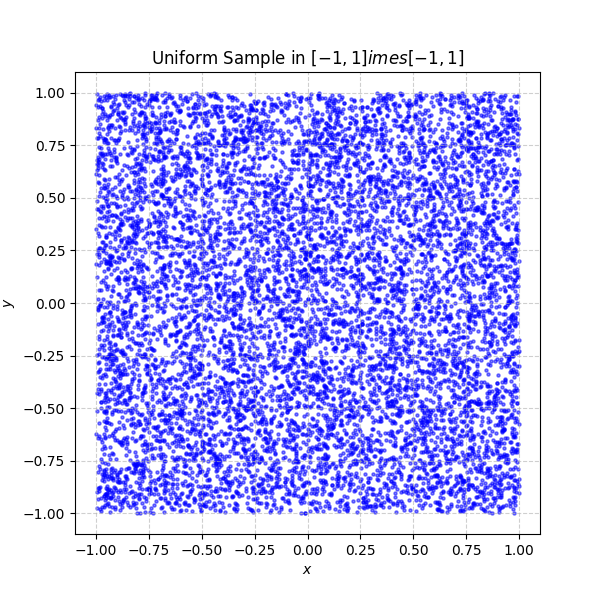
\includegraphics[width=\textwidth]{tex/ims/unixy.png}
    \end{minipage}
    \begin{minipage}{.4\textwidth}
    \centering
    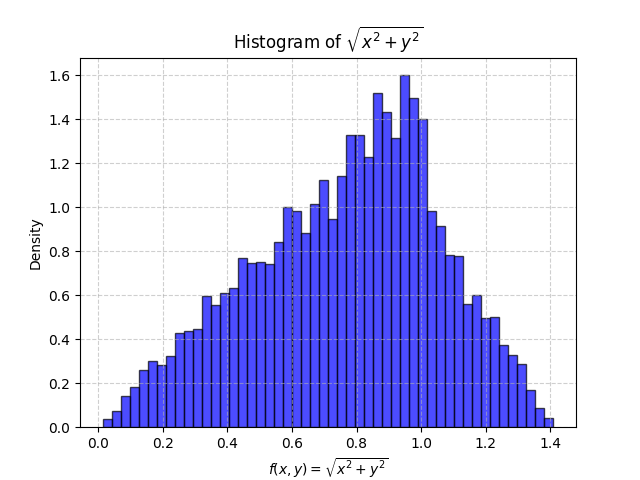
\includegraphics[width=\textwidth]{tex/ims/unirad.png}
    
    \end{minipage}
     \caption{A function on a uniform distribution need not yield a uniform distribution. An easy example is the radius function.}
             \end{figure}

So, the first row makes sense. 
For the single channel phase space in the bottom row, the distribution on the left is very narrowly distributed to 90GeV. This is because we reject a lot of points in order to only include momenta relevant to the process. In theory, multiplying but the Jacobian, which encodes this change of phase region, should yield in the bottom right a distribution that looks like the top row. Clearly, this doesn't seem to be the case. This is because we don't have enough statistics to accurately reproduce the top row - we have rejected a large number of samples. If we increase the width of the $Z$ boson from 60Gev to say, 6000GeV, we can see the distributions start to match a bit more closely, as we are rejecting fewer points.

\begin{figure}[H]
    \centering
    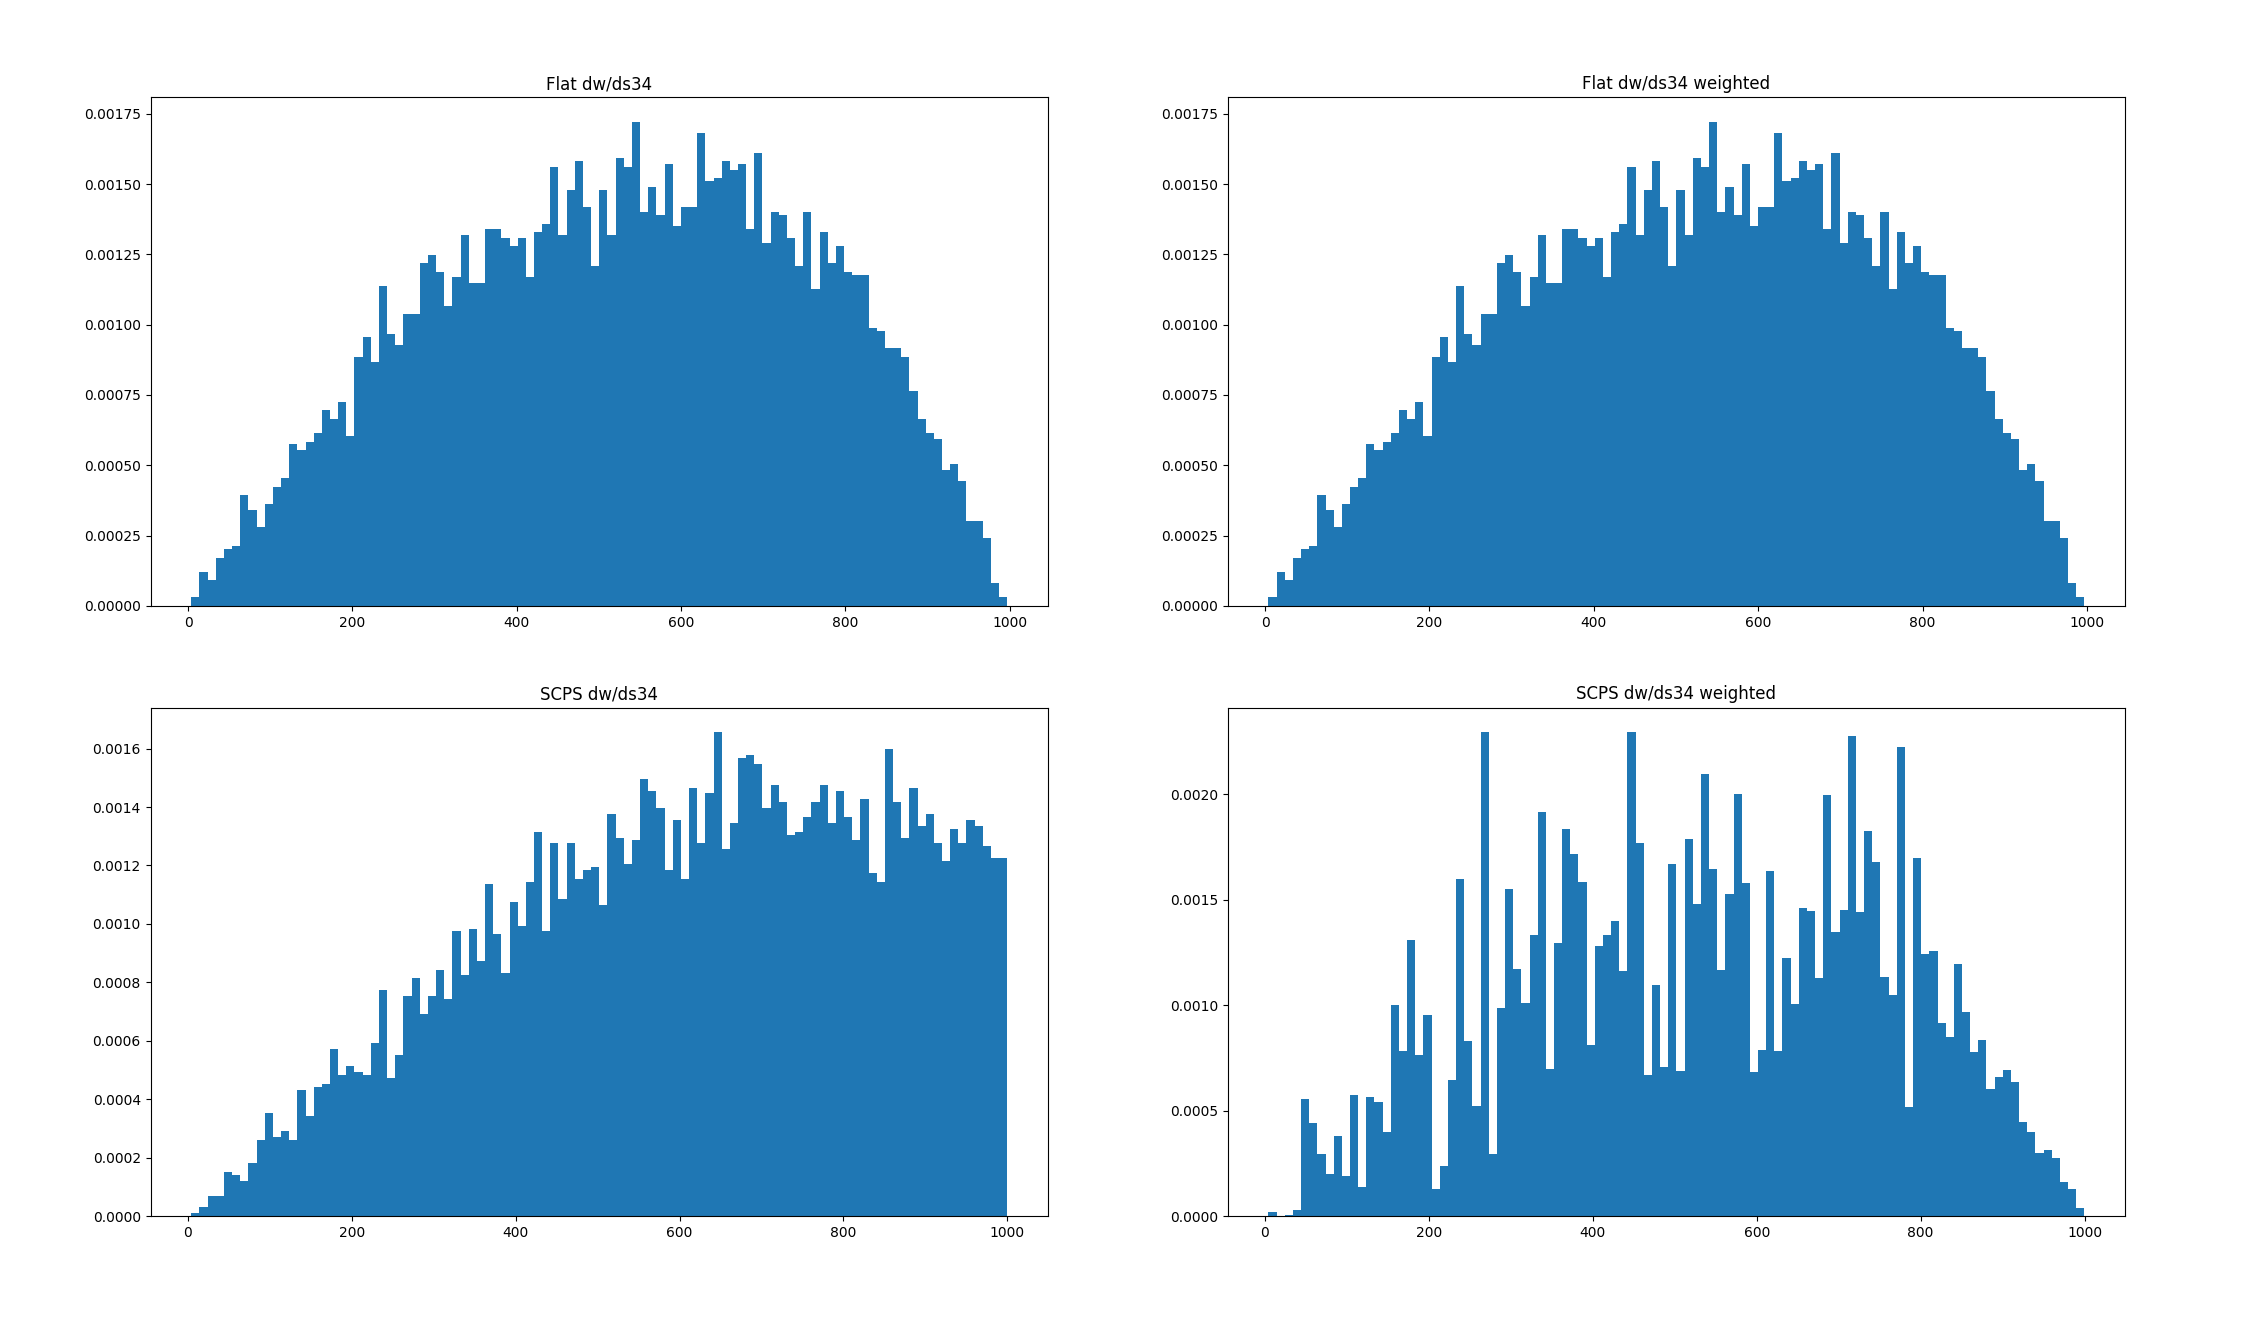
\includegraphics[width=0.75\linewidth]{tex/ims/phasespace2.png}
    \caption{Phase Space Sampling with the $Z$ boson with mass 150GeV and width 6000GeV. The reweighted distribution on the bottom right starts to look more like the top row, as with this width we reject fewer points and thus have better statistics.}
    \label{fig:phase2}
\end{figure}



% We can do this using Symbolica.
